\documentclass[sigconf]{acmart}
\usepackage{graphicx}
\usepackage{algorithmic}
\usepackage{algorithm}

%% Rights management information.  This information is sent to you
%% when you complete the rights form.  These commands have SAMPLE
%% values in them; it is your responsibility as an author to replace
%% the commands and values with those provided to you when you
%% complete the rights form.
\setcopyright{acmlicensed}
\copyrightyear{2025}
\acmYear{2025}
\acmConference[Algorithms Conference '25]{Proceedings of the Algorithms Conference '25}{May 20-June 3,
  2025}{Ljubljana, Slovenia}
\acmISBN{978-1-4503-XXXX-X/25/05}
\acmDOI{10.1145/XXXXXXX.XXXXXXX}

\acmArticleType{Review}

\title{Verifying Groups in Linear Time}

\author{Vanja Stojanovi\'c}
\email{vs66277@student.uni-lj.si}
\authornote{Corresponding author.}
\affiliation{
  \institution{University of Ljubljana}
  \department{Faculty of Mathematics and Physics}
  \city{Ljubljana}
  \country{Slovenia}
}

\author{Bor Panger\v si\v c}
\affiliation{
  \institution{University of Ljubljana}
  \department{Faculty of Mathematics and Physics}
  \city{Ljubljana}
  \country{Slovenia}
}

%— Authors from FRI —%
\author{Pia Sotlar}
\affiliation{
  \institution{University of Ljubljana}
  \department{Faculty of Computer Science and Informatics}
  \city{Ljubljana}
  \country{Slovenia}
}

\author{Klemen Kav\v ci\v c}
\affiliation{
  \institution{University of Ljubljana}
  \department{Faculty of Computer Science and Informatics}
  \city{Ljubljana}
  \country{Slovenia}
}

\keywords{Groups, Computational group theory, Cayley tables}

\begin{abstract}
  \bfseries
  This paper reviews the contributions of \cite{10756141}, which presents a deterministic \(O(n^2)\) algorithm for verifying whether an \(n \times n\) Cayley table defines a valid group. We analyze the key techniques—4-associativity, basis sets, and group decomposition—and discuss their implications for computational group theory and applications in cryptography and coding theory \cite{zurekCodingTheory}.
  \normalfont
\end{abstract}


\begin{document}

\maketitle


\section{Introduction}

\subsection{Problem Statement}
We examine the problem of verifying group axioms for a Cayley table, as addressed in \cite{10756141}. Their work establishes the first deterministic \(O(n^2)\) algorithm, improving prior brute-force and probabilistic methods.
\\A Cayley table for a set \(S\) of size \(n\) and operation \(\cdot\) is an \(n \times n\) matrix where entry \((i,j)\) equals \(s_i \cdot s_j\). The table defines a group if the following conditions hold:

\begin{enumerate}
    \item \textbf{Identity}: \(\exists e \in S\) such that \(e \cdot s = s \cdot e = s\) for all \(s \in S\).
    \item \textbf{Inverses}: \(\forall s \in S\), \(\exists s^{-1} \in S\) with \(s \cdot s^{-1} = s^{-1} \cdot s = e\).
    \item \textbf{Associativity}: \((a \cdot b) \cdot c = a \cdot (b \cdot c)\) for all \(a,b,c \in S\).
\end{enumerate}

\begin{example}
For \(\mathbb{Z}_3\) under addition:
\[
\begin{array}{|c|ccc|}
\hline
+ & 0 & 1 & 2 \\ \hline
0 & 0 & 1 & 2 \\
1 & 1 & 2 & 0 \\
2 & 2 & 0 & 1 \\ \hline
\end{array}
\]
Here \(0\) is the identity, and inverses are \(0^{-1}=0\), \(1^{-1}=2\), \(2^{-1}=1\).
\end{example}
Given an \( n \times n \) multiplication table, the goal is to determine if it represents a valid group.

\subsection{Motivation}
Verifying whether a given multiplication table defines a group is a fundamental problem in computational algebra with applications in cryptography, error-correcting codes and symbolic computation. The key challenge lies in efficiently checking the associativity axiom, which naively requires testing all possible triplets \((a, b, c)\) to ensure:
\[
(a \cdot b) \cdot c = a \cdot (b \cdot c).
\]
A brute-force approach would require \(O(n^3)\) time, which is impractical for large \(n\). While prior work has improved this to \(O\left(\frac{\log(1/\delta)}{\epsilon}\right).\) probabilistically, the question whether this can be removed has been open for some time.

\subsubsection*{Why Linear Time is Non-Obvious}
A natural hope might be that associativity could be verified in subcubic or linear time by exploiting algebraic structure. Associativity a priori seems to demand verification over all \(O(n^3)\) triplets, as the operation's behavior on one subset of elements need not constrain its behavior elsewhere. In \cite{verificationOfIdentities}, Rajagopalan and Schulman discuss this exact problem and show that for certain types of operations, a random algorithm works with high probability. However, as demonstrated by the following theorem, the random sampling approach cannot work in general as non-associativity can be "hidden" in a single triplet, even while the operation appears associative everywhere else.



\begin{theorem}[Local Non-Associativity]
On every set with at least 4 elements, there exists a binary operation that is associative everywhere except on one triplet.
\end{theorem}
\begin{proof}
Let \( S \) be a set with \( |S| \geq 4 \). Choose distinct elements \( a, u, v, w \in S \). Define a binary operation \( * \) on \( S \) as follows:
\[
x * y =
\begin{cases}
u & \text{if } x = a \text{ and } y = a, \\
v & \text{if } x = a \text{ and } y = u, \\
w & \text{otherwise}.
\end{cases}
\]
We claim \( * \) is associative except for the triplet \( (a, a, a) \).
\\
\textbf{Non-associativity at \( (a, a, a) \):}
\[
(a * a) * a = u * a = w, \quad \text{but} \quad a * (a * a) = a * u = v.
\]
Since \( w \neq v \), \( (a * a) * a \neq a * (a * a) \).
\\
\textbf{Associativity for all other triplets:}
\\
First, let's analyze LHS $=(x \ast y) \ast z$. Let $p_1 = x \ast y$.
\begin{itemize}
    \item If $(x,y) = (a,a)$, then $p_1 = u$. LHS $= u \ast z$.
    Since $u \neq a$, the pair $(u,z)$ is neither $(a,a)$ nor $(a,u)$. So, $u \ast z = w$ by definition (3).
    \item If $(x,y) = (a,u)$, then $p_1 = v$. LHS $= v \ast z$.
    Since $v \neq a$, the pair $(v,z)$ is neither $(a,a)$ nor $(a,u)$. So, $v \ast z = w$ by definition (3).
    \item If $(x,y) \neq (a,a)$ and $(x,y) \neq (a,u)$, then $p_1 = w$. LHS $= w \ast z$.
    Since $w \neq a$, the pair $(w,z)$ is neither $(a,a)$ nor $(a,u)$. So, $w \ast z = w$ by definition (3).
\end{itemize}
In all possible cases for $(x,y)$, LHS $=(x \ast y) \ast z = w$.
\\
Next, let's analyze RHS $= x \ast (y \ast z)$. Let $p_2 = y \ast z$.
\begin{itemize}
    \item If $(y,z) = (a,a)$, then $p_2 = u$. RHS $= x \ast u$.
    \begin{itemize}
        \item If $x = a$, this corresponds to the triplet $(a,a,a)$. As shown before, RHS $= a \ast u = v$.
        \item If $x \neq a$, the pair $(x,u)$ is not $(a,a)$ (since $x \neq a$) and not $(a,u)$ (since $x \neq a$). So, $x \ast u = w$ by definition (3).
    \end{itemize}
    \item If $(y,z) = (a,u)$, then $p_2 = v$. RHS $= x \ast v$.
    Since $v \neq a$ and $v \neq u$ (as $a,u,v,w$ are distinct), the pair $(x,v)$ cannot be $(a,a)$ (as $v \neq a$) and cannot be $(a,u)$ (as $v \neq u$). So, $x \ast v = w$ by definition (3).
    \item If $(y,z) \neq (a,a)$ and $(y,z) \neq (a,u)$, then $p_2 = w$. RHS $= x \ast w$.
    Since $w \neq a$ and $w \neq u$ (as $a,u,v,w$ are distinct), the pair $(x,w)$ cannot be $(a,a)$ (as $w \neq a$) and cannot be $(a,u)$ (as $w \neq u$). So, $x \ast w = w$ by definition (3).
\end{itemize}

\end{proof}

\subsection{Applications of the Finding and Usage of Cayley Tables}

Within computational group theory software, such as GAP and Magma, efficient Cayley table verification plays a foundational role.
These systems allow users to define finite groups by providing their Cayley tables.
Upon input, the software must verify if the given table adheres to the group axioms (closure, associativity, identity, and inverses)
before allowing further computations or analysis. 

For instance, if a user intends to find the subgroups, conjugacy classes, or
other properties of a group defined by its Cayley table, the system first needs to ensure that the input indeed represents a valid group. 
Efficient verification algorithms make this initial validation process practical, especially for groups of moderate size. 
Furthermore, while not the most scalable approach for very large groups, Cayley tables can be employed in group isomorphism 
testing, particularly for groups with a smaller number of elements \cite{williams2015group}.

Finite groups also play a role in coding theory, particularly in the construction of error-correcting codes. For example, cyclic codes have a close 
relationship with cyclic groups. The algebraic properties of the underlying group often determine the characteristics and error-correcting
capabilities of these codes. The study of perfect codes (subsets of a graph with specific distance properties relevant to error correction)
sometimes involves Cayley graphs of groups.

In such contexts, verifying the group structure ensures that the Cayley graph possesses
the intended properties necessary for code construction and analysis. Additionally, research explores the construction of generator
and parity check matrices for error-correcting codes directly from the Cayley tables of certain algebraic structures \cite{zurekCodingTheory}.

\subsection{Prior Work}
To satisfy the third property of Cayley tables (associativity) we would have to check all triples. So to check for associativity, or more precisely that for every \(a,b,c  \in S\) it holds that \((a\times b)\times c = a\times (b\times c)\) a brute force algorithm would require \(\Theta(n^3)\) time. Before the linear-time algorithm, two other methods for checking associativity were proposed \cite{10756141}.
\subsubsection{Light's \( O(n^2 \log n) \) deterministic method}
In 1949 Dr. F. W. Light noticed that we can check for associativity only for all triples a,b,c such that \(a,c \in S\) and \(b\in R\), where R is a set of generators of S. A generating set R is a set of elements from set S from which you can build all other elements in the set S with the use of group operation. 

For a finite set S and a binary operation \((\cdot)\) we can define two operations:

\[a * c = a\cdot(b\cdot c)\] and
\[a \circ c= (a\cdot b)\cdot c\]

Associativity holds in S if for every element \(b \in R\) the operations \(*\) and \(\circ\) coincide for all \(a,c \in S\). We can do this reduction because if every element in S can be written as a combination of generators from R, and associativity is preserved, it is enough to verify associativity only on elements from R.
The general idea is to construct the Cayley tables for both operations and see if they are the same.

This method reduces the number of checks needed compared to checking all the combinations, because it avoids redundant computations. It checks associativity in \(\mathcal{O}(n^2logn)\) for R size \(logn\) and all \(a,c \in S\) \cite{clifford1961algebraic}.

\begin{table}[h]
\centering
\begin{tabular}{|c|c|c|c|c|c|}
\hline
\textbf{.} & \textbf{a} & \textbf{b} & \textbf{c} & \textbf{d} & \textbf{e} \\ \hline
\textbf{a} & a & a & a & d & d \\ \hline
\textbf{b} & a & b & c & d & d \\ \hline
\textbf{c} & a & c & b & d & d \\ \hline
\textbf{d} & d & d & d & a & a \\ \hline
\textbf{e} & d & e & e & a & a \\ \hline
\end{tabular}
\caption{Example Cayley Table}
\label{tab:example}
\end{table}

In Table~\ref{tab:example} \(\{c,e\}\) is the generating set. For c, the procedure is shown in Figure ~\ref{fig:procedure} below. We copy the c-row and c-column from the original table into new tables as the top and left headers. For each element in the header, we copy the corresponding column or row from the original table. To prove that associativity holds, we compare the tables * (c) and ° (c). If they are the same, associativity holds for c. Repeating this for all generators confirms associativity for the whole set \cite{clifford1961algebraic}.

\begin{figure}[H]
    \centering
    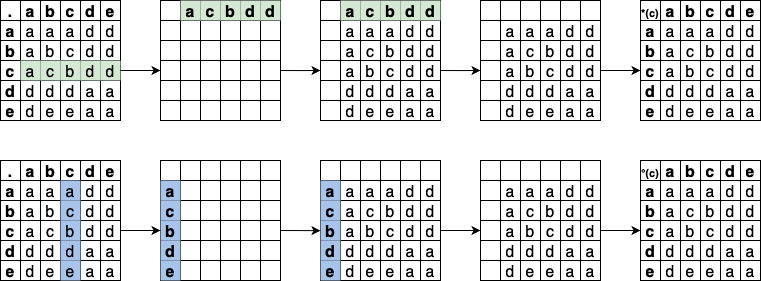
\includegraphics[width=1\linewidth]{Lights.png}
    \caption{Procedure for Light's associativity test}
    \label{fig:procedure}
\end{figure}

\subsubsection{Rajagopalan \& Schulman's randomized \( O(n^2 \log(1/\delta)) \).}
Rajagopalan and Schulman \cite{548520} develop a randomized method, which achieves running time $O(n^2 \log(1/\delta))$, where $\delta$ is the allowed error probability. This reduces the time from cubic to nearly quadratic, making the approach much more efficient for large sets.
Instead of checking all possible triplets in the set, the method randomly samples a carefully chosen number of triples and tests whether the associativity condition holds for each sampled combination. By choosing the number of samples carefully, they can detect non-associativity with high probability, even though they do not check every combination.
The number of random samples $k$ is determined based on the desired error probability $\delta$:
\[k = O\left(\frac{\log(1/\delta)}{\epsilon}\right).\]
Here, $\epsilon$ is the (unknown) fraction of triples where associativity fails. 
The method guarantees that if the operation is non-associative and enough triples fail, the probability of missing all failing triples after sampling is at most $\delta$. This makes the algorithm particularly useful when working with large data, where deterministic checking is computationally too expensive. It allows researchers to balance speed and confidence: they can choose the acceptable error $\delta$ and get a provably good result much faster than with deterministic methods.
However, the efficiency depends on having a good understanding or estimate of the expected error $\epsilon$ in the table. If the number of failing triples is very small, the method may not be much more efficient than brute-force checking.
Rajagopalan and Schulman’s method achieves complexity that is better than the one implied by Light’s observation when we allow a nonzero error probability $\delta$. However, the downside is that it does use randomness and introduces some probability of error.
    

\subsection{Contributions}
\begin{itemize}
    \item First deterministic \( O(n^2) \) algorithm.
    \item Use of \textbf{basis sets} and \textbf{4-associativity}.
    \item Reduction in the search for large subgroups by group decomposition.
\end{itemize}

\section{Technical Overview}
\subsection{Testing Group Axioms with Brute Force Methods}
When given a multiplication table (Cayley table) of a set $S$, we can check whether it has an identity element and inverses by brute force by systematically scanning the table. Each of these processes takes $O(n^2)$ time, where $n$ is the size of the set.

\begin{algorithm}[H]
\caption{Brute-Force Identity Element Verification}
\begin{algorithmic}[1]
\REQUIRE Cayley table for set $S$ of size $n$
\ENSURE Identity element $e$ or $\emptyset$ if none exists
\FOR{each element $e \in S$}
    \STATE $is\_identity \gets \text{TRUE}$
    \FOR{each element $g \in S$}
        \IF{$e \cdot g \neq g$ OR $g \cdot e \neq g$}
            \STATE $is\_identity \gets \text{FALSE}$
            \STATE $\textbf{break}$
        \ENDIF
    \ENDFOR
    \IF{$is\_identity$}
        \RETURN $e$
    \ENDIF
\ENDFOR
\STATE \RETURN $\emptyset$
\end{algorithmic}
\end{algorithm}

\begin{proposition}
The brute-force identity verification requires \( O(n^2)\) operations.
\end{proposition}

\begin{proof}
For each of the $n$ candidate elements $e\in S$, we must verify the identity property against all n elements $g \in S$. Each verification requires checking two multiplications, resulting in exactly $2n$ operations in the worst case.
\end{proof}



\begin{algorithm}[H]
\caption{Brute-Force Inverse Elements Verification}
\begin{algorithmic}[1]
\REQUIRE Cayley table for set $S$ of size $n$, identity element $e$
\ENSURE TRUE if all elements have inverses, FALSE otherwise
\FOR{each element $g \in S$}
    \STATE $inverse\_found \gets \text{FALSE}$
    \FOR{each element $h \in S$}
        \IF{$g \cdot h = e$ AND $h \cdot g = e$}
            \STATE $inverse\_found \gets \text{TRUE}$
            \STATE $\textbf{break}$
        \ENDIF
    \ENDFOR
    \IF{NOT $inverse\_found$}
        \RETURN FALSE
    \ENDIF
\ENDFOR
\STATE \RETURN TRUE
\end{algorithmic}
\end{algorithm}

\begin{proposition}
The brute-force inverse verification requires $O(n^2)$ operations.
\end{proposition}

\begin{proof}
For each of the $n$ elements $g \in S$, we search through up to $n$ potential inverses $h \in S$, with each candidate requiring two multiplication checks. This yields a worst-case complexity of $2n^2$ operations.
\end{proof}

\subsection{Testing Group Axioms Efficiently}
We present efficient algorithms for verifying the identity and inverse axioms of a group given its multiplication table as mentioned in \cite{10756141}. While brute-force approaches require $O(n^2)$ time for these checks, we demonstrate how to reduce this to $O(n\log n)$ time.

\subsubsection{Identity Element Verification}

\begin{theorem}
Given a finite set $G$ of size $n$ with a binary operation, the identity element $e \in G$, if it exists, can be found and verified in $O(n)$ time.
\end{theorem}

\begin{proof} The identity verification proceeds in two phases:

1. \textbf{Candidate Identification:} We search for an element $e \in G$ satisfying $e \cdot e = e$. This requires checking $n$ elements with one operation each, yielding $O(n)$ time.

2. \textbf{Identity Validation:} For the candidate $e$, we verify that $e \cdot g = g \cdot e = g$ for all $g \in G$. This requires $2n$ checks (examining both the row and column of $e$ in the multiplication table), maintaining $O(n)$ complexity.

The uniqueness of $e$ follows from standard group theory: if $e'$ were another identity, we would have $e = e \cdot e' = e'$.
\end{proof}

\subsubsection{Inverse Elements Verification}

\begin{theorem}
Assuming associativity, the existence of inverses for all elements in $G$ can be verified in $O(n\log n)$ time.
\end{theorem}

\begin{proof}
For each $g \in G$, we compute its inverse as $g^{-1} = g^{n-1}$ using the following method:

1. \textbf{Exponentiation by Squaring:} For each element $g$, compute $g^{n-1}$ in $O(\log n)$ time through repeated squaring. This relies on the associativity of the operation.

2. \textbf{Inverse Verification:} For each $g$, confirm that $g \cdot g^{n-1} = e$ in $O(1)$ time per element.

The total time complexity is $O(n\log n)$. The correctness follows from Lagrange's theorem for finite groups, where $g^{|G|} = e$ for any $g \in G$.
\end{proof}

\subsubsection{Example Application}
\label{subsec:example}

Consider the group $G = \{1, i, -1, -i\}$ under complex multiplication. We demonstrate our algorithms:

\begin{enumerate}
    \item \textbf{Identity Finding:} The only element satisfying $e \cdot e = e$ is $1$. Verification shows $1 \cdot g = g \cdot 1 = g$ for all $g \in G$.

    \item \textbf{Inverse Computation:} For $n=4$, we compute:
    \begin{align*}
        1^{-1} &= 1^3 = 1 \\
        i^{-1} &= i^3 = -i \\
        (-1)^{-1} &= (-1)^3 = -1 \\
        (-i)^{-1} &= (-i)^3 = i
    \end{align*}
    Each computation requires $O(\log n)$ operations, with all inverses verifying correctly against the identity.
\end{enumerate}

\subsubsection{Complexity Analysis}

Table~\ref{tab:complexity} compares the brute-force and optimized approaches:

\begin{table}[h]
\centering
\caption{Time complexity comparison for group axiom verification}
\label{tab:complexity}
\begin{tabular}{lcc}
\hline
Operation & Brute-Force & Optimized \\
\hline
Identity Verification & $O(n^2)$ & $O(n)$ \\
Inverse Verification & $O(n^2)$ & $O(n\log n)$ \\
\hline
\end{tabular}
\end{table}



\subsection{4-Associativity and Basis Sets}
To verify if for a given operation on a set G is associative, many methods have been proposed. Light proposed a method that reduces the runtime of the \(\mathcal{O}(n^3)\) brute force approach to \(\mathcal{O}(n^2log(n))\), while Rajagopalan and Schulman developed a randomized algorithm which achieves running time $O(n^2 \log(1/\delta))$. Prior to this work, no other method had managed to reach a faster running time.

\subsubsection{Basis and 4-associativity Definition}
\begin{definition}
If G is a set with a binary operation \(\cdot\): G×G→G, then a subset S of G is said to be a basis of G if $S\cdot S := \{s1\cdot s2 |s1,s2 \in S\}$ while $|S|\le3\sqrt{|G|}$.
\end{definition}

The operation \(\cdot\) is said to be 4-associative over a set S, if for all $a,b,c,d \in S$ we have $((ab)c)d= (ab)(cd) = (a(bc))d= a((bc)d) = a(b(cd))$.

\subsubsection{Key Lemma}
If \(\cdot\) is 4-associative over S, then \(\cdot\) is associative over G.

\textbf{Proof (Adapted from \cite{10756141})}:
To prove 4-associativity over G, we first define \(\alpha, \beta,\gamma \in G\). There exist elements \(a,b,c,d,e,f \in S\) such that
\[\alpha = ab,\]
\[\beta = cd,\]
\[\gamma = ef.\]


In order to show \( G \) is associative, we must prove
\begin{equation}
((ab)(cd))(ef) = (\alpha \cdot \beta) \cdot \gamma = \alpha \cdot (\beta \cdot \gamma) = (ab)((cd)(ef)). \tag{1}
\end{equation}

Since \( G = S \cdot S \), we can write
\[
b(cd) = uv, \quad a(uv) = wx, \quad (cd)e = st, \quad (st)f = pq, \quad (b(cd))e = yz,
\]
with \( p, q, s, t, u, v, w, x, y, z \in S \). Using this, and 4-associativity of \( \cdot \) on \( S \), we get that
\begin{align}
((ab)(cd))(ef) &= (a(b(cd)))(ef) = (wx)(ef) = ((wx)e)f \notag \\
&= ((a(uv))e)f = (a((uv)e))f = (a((b(cd))e))f. \tag{2}
\end{align}

Completely symmetrically, if we reflect all parentheses, we get
\begin{align}
(ab)((cd)(ef)) &= ab(((cd)e)f) = ab(pq) = a(b(pq)) \notag \\
&= a(b((st)f)) = a((b(st))f) = a((b((cd)e))f). \tag{3}
\end{align}

Finally, we show that the right-hand sides of (2) and (3) are equal, to deduce (1):
\[
(a((b(cd))e))f = (a(yz))f = a((yz)f) = a(((b(cd))e)f) = a((b((cd)e))f).
\]

Because we enumerate all sets of four elements of S ($|S| = O(\sqrt{n})$), we can check for 4-associativity in $\mathcal{O}\left((n^{1/2})^4\right) = \mathcal{O}(n^2)$ time.

\subsection{Reduction to Finding Large Subgroups}
\label{sec:large-subgroups}

%\subsubsection{Overview}
The core challenge in this subsection is constructing a \emph{basis} $S \subseteq G$ with $|S| = O(\sqrt{n})$ and $S^2 = G$, which enables efficient associativity testing via 4-associativity. The authors show that this reduces to finding \emph{large subgroups} $H \leq G$ where $|H| \geq \sqrt{|G|}$.

\begin{definition}[Large Subgroup]
A proper subgroup $H \leq G$ is \textbf{large} if $\sqrt{|G|} \leq |H| < |G|$.
\end{definition}

\begin{definition}[Group Decomposition]
For a group $G$ of size $n$ and parameter $\ell$, an \textbf{$\ell$-decomposition} is a pair $(A,B)$ where:
\begin{itemize}
    \item $A \cdot B = G$
    \item $|A| \leq 2\ell$
    \item $|B| \leq n/\ell$
\end{itemize}
\end{definition}

The reduction proceeds via three main phases:

\textbf{Phase 1: Recursive Decomposition}
Given a large subgroup $H$, we recursively decompose $G$:
\begin{itemize}
    \item \textbf{Base Case}: If $G$ is cyclic of prime order, use arithmetic progressions.
    \item \textbf{Recursive Case}:
    \begin{enumerate}
        \item If $|H| \geq n/(2\ell)$, set $A$ as a left transversal of $H$, $B = H$.
        \item Else, recursively decompose $H$ and lift to $G$ via transversals.
    \end{enumerate}
\end{itemize}

\begin{algorithm}[H]
\caption{GroupDecomposition}
\begin{algorithmic}[1]
%\Require Group $G$, parameter $\ell$
\IF{$|G|$ is prime}
    \STATE Return cyclic decomposition
\ELSE
    \STATE $H \gets \text{LargeSubgroup}(G)$
    \IF{$|H| \geq n/(2\ell)$}
        \STATE $A \gets \text{LeftTransversal}(G,H)$
        \STATE $B \gets H$
    \ELSE
        \STATE $(A',B') \gets \text{GroupDecomposition}(H,\ell)$
        \STATE $A \gets A'$
        \STATE $B \gets B' \cdot \text{RightTransversal}(G,H)$
    \ENDIF
\ENDIF
\RETURN $(A,B)$
\end{algorithmic}
\end{algorithm}

\textbf{Phase 2: Transversal Computation}
\begin{lemma}[Left Transversal]
A left transversal $T$ of $H \leq G$ can be found in $O(n)$ time by:
\begin{enumerate}
    \item Greedily selecting representatives from distinct cosets
    \item Removing entire cosets after selection
\end{enumerate}
\end{lemma}

\textbf{Phase 3: Basis Construction}
\begin{corollary}
Setting $\ell = \sqrt{n/2}$ yields a basis $S = A \cup B$ with $|S| \leq 2\sqrt{2n} < 3\sqrt{n}$.
\end{corollary}


\subsection{Reduction to Simple Groups}
\label{sec:simple-groups}

The algorithm reduces the large subgroup search problem to the case of \emph{simple groups} by:
\begin{itemize}
    \item Finding normal subgroups efficiently
    \item Recursively processing quotient groups
    \item Handling simple groups as base cases
\end{itemize}

\begin{definition}[Simple Group]
A group \( G \) is \textbf{simple} if its only normal subgroups are \( \{e\} \) and \( G \) itself.
\end{definition}

\subsubsection{Identifying normal subgroups}
The algorithm identifies normal subgroups through:

\textbf{Step 1: Small Generating Set}
\begin{itemize}
    \item Compute a generating set \( S \) with \( |S| \leq \log|G| \) in \( \widetilde{O}(n) \) time
    \item Uses greedy expansion of non-generator elements
\end{itemize}

\begin{algorithm}[H]
\caption{Generators}
\begin{algorithmic}[1]
\STATE \( H \gets \{e\} \)
\STATE \( S \gets \emptyset \)
\FOR{each \( a \in A \)}
    \IF{\( a \notin H \)}
        \STATE \( S \gets S \cup \{a\} \)
        \STATE \( H \gets \langle S \rangle \)
    \ENDIF
\ENDFOR
\RETURN \( S \)
\end{algorithmic}
\end{algorithm}

\textbf{Step 2: Conjugacy Class Graph}
\begin{itemize}
    \item Build graph where vertices are conjugacy classes
    \item Edge \( C_i \to C_j \) if elements from \( C_i \) multiply into \( C_j \)
    \item Compute in \( \widetilde{O}(n) \) time using generators
\end{itemize}

\textbf{Step 3: Closed Union Detection}
\begin{itemize}
    \item Normal subgroups correspond to closed unions of classes
    \item Dynamically maintain reachability in the graph
\end{itemize}

\subsubsection{Recursive Reduction}
\begin{lemma}[6.2]
Given an algorithm for simple groups, LargeSubgroup runs in \( O(n^{3/2+\epsilon}) \) time for arbitrary groups.
\end{lemma}

\begin{algorithm}[H]
\caption{LargeSubgroup}
\begin{algorithmic}[1]
\STATE \( N \gets \text{NormalSubgroup}(G) \)
\IF{\( N = G \)}
    \RETURN \(\text{LargeSubgroupOfSimpleGroup}(G)\)
\ELSIF{\( |N| \geq \sqrt{n} \)}
    \RETURN \( N \)
\ELSIF{\( G/N \) has prime order}
    \STATE Find element \( g \) of prime order \( p \)
    \RETURN \( \langle g \rangle \)
\ELSE
    \STATE \( M \gets \text{LargeSubgroup}(G/N) \)
    \RETURN \( M \cdot N \)
\ENDIF
\end{algorithmic}
\end{algorithm}

\subsubsection{Complexity Analysis}
\begin{itemize}
    \item Normal subgroup finding: \( \widetilde{O}(n) \) via dynamic graph maintenance
    \item Recursion depth: \( O(\log n) \) (each step reduces problem size)
    \item Bottleneck: Simple group handling (\( O(n^{3/2+\epsilon}) \))
\end{itemize}

\begin{theorem}
The reduction to simple groups preserves the overall \( O(n^{3/2+\epsilon}) \) time complexity when combined with:
\begin{itemize}
    \item \( \widetilde{O}(n) \) normal subgroup detection
    \item \( O(n^{3/2+\epsilon}) \) simple group processing
\end{itemize}
\end{theorem}

\subsection{Finding Large Subgroups of Simple Groups}
\label{sec:simple-subgroups}

The algorithm handles simple groups through a classification-based approach:

\begin{definition}[Simple Group Types]
Finite simple groups fall into three categories:
\begin{itemize}
    \item Cyclic groups of prime order
    \item Alternating groups $A_n$ ($n \geq 5$)
    \item Groups of Lie type and sporadic groups
\end{itemize}
\end{definition}

\subsubsection{Classification Strategy}
\begin{itemize}
    \item \textbf{Step 1: Group Identification} - Enumerate possible isomorphisms:
    \begin{algorithm}[H]
    \caption{EnumerateGroups}
    \begin{algorithmic}[1]
    \FOR{each simple group family $f$}
        \STATE Solve $|f(m,q)| = n$ for parameters $(m,q)$
        \IF{solution exists}
            \STATE Add $(f,m,q)$ to candidate list
        \ENDIF
    \ENDFOR
    \RETURN candidates
    \end{algorithmic}
    \end{algorithm}
    
    \item \textbf{Step 2: Type-Specific Handling} - Different approaches per category
\end{itemize}

\subsubsection{Algorithmic Approaches}

\textbf{Case 1: Alternating Groups ($A_n$)}
\begin{itemize}
    \item Find the natural subgroup $A_{n-1}$
    \item Implementation steps:
    \begin{enumerate}
        \item Identify all 3-cycles (elements of order 3)
        \item Find a set conjugate to $\{(1,2,k) | 3 \leq k \leq n\}$
        \item Remove one generator to get $A_{n-1}$
    \end{enumerate}
    \item Runtime: $\widetilde{O}(n)$
\end{itemize}

\textbf{Case 2: Groups of Lie Type}
\begin{itemize}
    \item Key tool: Borel subgroups
    \begin{definition}[Borel Subgroup]
    A maximal connected solvable subgroup.
    \end{definition}
    
    \item Implementation:
    \begin{algorithm}[H]
    \caption{BorelSubgroup}
    \begin{algorithmic}[1]
    \STATE Find Sylow $p$-subgroup $P$ (char. $p$ of field)
    \STATE Compute normalizer $B = N_G(P)$
    \RETURN $B$
    \end{algorithmic}
    \end{algorithm}
    
    \item Construct parabolic subgroup:
    \begin{itemize}
        \item Find element $a$ such that $P = \langle B, a \rangle$ is large
        \item Verify $|P| \geq \sqrt{|G|}$
    \end{itemize}
    \item Runtime: $O(n^{3/2+\epsilon})$
\end{itemize}

\textbf{Case 3: Sporadic Groups}
\begin{itemize}
    \item Finite list of 26 exceptions + Tits group
    \item Precomputed large subgroups from group theory literature
    \item Constant-time lookup
\end{itemize}

\subsubsection{Theoretical Guarantees}
\begin{theorem}[Existence]
Every non-prime simple group contains a large subgroup.
\end{theorem}

\begin{proof}[Proof Sketch]
\begin{itemize}
    \item Alternating: $|A_{n-1}| \geq \sqrt{|A_n|}$
    \item Lie type: Parabolic subgroups satisfy size requirement
    \item Sporadic: Verified case-by-case
\end{itemize}
\end{proof}

\subsubsection{Complexity Analysis}
\begin{itemize}
    \item Alternating groups: $\widetilde{O}(n)$ (dominated by 3-cycle detection)
    \item Lie type: $O(n^{3/2+\epsilon})$ (Borel subgroup construction)
    \item Sporadic: $O(1)$ (table lookup)
    \item Classification: $O(\log^4 n)$ (parameter solving)
\end{itemize}

\begin{lemma}
The simple group handling preserves the overall $O(n^{3/2+\epsilon})$ time complexity.
\end{lemma}

% 3. Critical Analysis (3–4 pages)
\section{Critical Analysis}

\subsection{Limitations}

The algorithm's method for handling simple groups, a crucial step in its group decomposition strategy (Section~\ref{sec:simple-subgroups}), relies significantly on the Classification of Finite Simple Groups (CFSG)~\cite{Aschbacher2004Notices}. In particular, for the 26 sporadic groups, the approach involves a ``constant-time lookup'' of precomputed data, such as their large subgroups~\cite{Conway1985Atlas, Wilson2009Simple}, rather than deriving these properties algorithmically from the input Cayley table using a general procedure. This reliance on an exhaustive list of known exceptions and their externally established properties means that, while effective for all currently known finite simple groups, this specific part of the algorithm is not self-contained in its treatment of sporadic groups. 

\subsection{Open Problems}
Building on the core insight from~\cite{10756141}---that 4-associativity on a carefully constructed basis \(S\) (where \(S \cdot S = G\)) implies global associativity for \(G\)---another compelling open problem emerges. The authors of~\cite{10756141} themselves suggest that this observation, despite its direct proof, "could be useful elsewhere." This motivates a broader exploration of such "k-tuple tests on a basis" for verifying other algebraic identities or properties. Key questions include: 
\begin{itemize}
    \item For which other fundamental algebraic identities (e.g., distributivity in rings, the Jacobi identity in Lie algebras, or various identities defining specific varieties of loops or semigroups~\cite{Bruck1971SurveyBinary, CliffordPreston1961Vol1}) can one establish a minimal integer \(k\) and a corresponding definition of a "basis" such that a \(k\)-tuple version of the identity holding on this basis guarantees the global identity? 
    \item How do the requisite properties of such a basis (e.g., covering conditions like \(S^k = G\)) and the value of \(k\) depend on the algebraic structure and the specific identity being tested~\cite{BurrisSankappanavar1981UniversalAlgebra}?
    \item Could this local-to-global paradigm lead to new efficient, deterministic verification algorithms in contexts where current methods are predominantly probabilistic~\cite{verificationOfIdentities, 548520} or necessitate more exhaustive checks, such as certain instances of the word problem in groups or semigroups~\cite{LyndonSchupp1977Combinatorial}?
\end{itemize}
Answering these questions could significantly advance the toolkit for algorithmic verification of properties in diverse algebraic settings.

\section{Conclusion}
The algorithm achieves $O(n^2)$ time complexity, matching the $\Omega(n^2)$ lower bound for Cayley table verification. This resolves the long-standing open problem of whether associativity can be verified in quadratic time deterministically, surpassing the $O(n^2 \log n)$ of Light's method and the probabilistic $O(n^2 \log(1/\delta))$ of Rajagopalan-Schulman. While its reliance on CFSG and hidden constants may limit immediate practicality, the novel use of 4-associativity and group decomposition opens avenues for future research in algorithm design and algebraic verification.

\bibliographystyle{ACM-Reference-Format}
\bibliography{references}

\end{document}

